\documentclass{article}
\usepackage{geometry}
\usepackage{xcolor}
\usepackage{graphicx}
\usepackage{float,lscape}
\usepackage{listings}
\usepackage{color}
\usepackage{lipsum}% Used for dummy text.
\definecolor{titlepagecolor}{cmyk}{1,.60,0,.40}
\definecolor{namecolor}{cmyk}{1,.50,0,.10}
\definecolor{dkgreen}{rgb}{0,0.6,0}
\definecolor{gray}{rgb}{0.5,0.5,0.5}
\definecolor{mauve}{rgb}{0.58,0,0.82}
\lstset{frame=tb,
  language=Java,
  aboveskip=3mm,
  belowskip=3mm,
  showstringspaces=false,
  columns=flexible,
  basicstyle={\small\ttfamily},
  numbers=none,
  numberstyle=\tiny\color{gray},
  keywordstyle=\color{blue},
  commentstyle=\color{dkgreen},
  stringstyle=\color{mauve},
  breaklines=true,
  breakatwhitespace=true,
  tabsize=3
}
%-----------------------------------------------------------------
\begin{document}
\thispagestyle{plain}
\begin{center}
    \Large
    EFM With Field in 111 Starting With Random and Ground Initial States
    
    \vspace{0.4cm}
    \large
    May 2nd, 2016 - May 18th, 2016
    
    \vspace{0.4cm}
    \textbf{Andrew Way}
    
    \vspace{0.9cm}
    \textbf{Overview} \\
    \vspace{5mm}
    The effective field method was used to 3000 iterations to determine the 0 temperature states of 
    the 12x12x12 3D FCC kagome lattice while being subjected to a changing magnetic field along the 111 
    direction. The field was either incremented or decremented in steps of 0.0001. 
    There were 4 cases studied:
    \begin{enumerate}
     \item \textbf{Increasing} magnetic field in the \textbf{111} direction from \textbf{0.00 to 0.05},
     with an initial 
     spin configuration that was a \textbf{ground state} with theta = 0.206275 and phi = 3.11867.
     \item \textbf{Increasing} magnetic field in the \textbf{111} direction from \textbf{0.00 to 0.05},
     with an initial 
     spin configuration that was \textbf{randomly generated}.
     \item \textbf{Decreasing} magnetic field in the \textbf{111} direction from \textbf{0.05 to 0.00},
     with an initial
     spin configuration that was a \textbf{ground state} with theta = 0.206275 and phi = 3.11867.
     \item \textbf{Decreasing} magnetic field in the \textbf{111} direction from \textbf{0.05 to 0.00},
     with an initial
     spin configuration that was \textbf{randomly generated}.
    \end{enumerate}
    Analysis that was performed on the resulting data included the following:
    \begin{itemize}
     \item Plots of magnetization versus field
     \item Plots of energy versus field
     \item Animations of the characteristic 6 spins 
     \item Determination of the number of ``unique'' spins that populate the lattice
     \item Determination of the components of the unique spins
     \item Plots of azimuth and zenith angles of the A, B, C, D, E, and F spins w.r.t. the plane of the 111 normal vector 
    \end{itemize}

\end{center}
\pagebreak
\thispagestyle{plain}
\begin{center}
\LARGE
RUN 1: Increasing Field, Ground State
\end{center}
\paragraph
\large
Steps persist in the energy graphs. This can probably be fixed by increasing precision. 
A sudden drop in energy occurs at field 0.0049. Little difference between the 2000 and 3000 step simulation.
\begin{figure}[h]
 \centering 
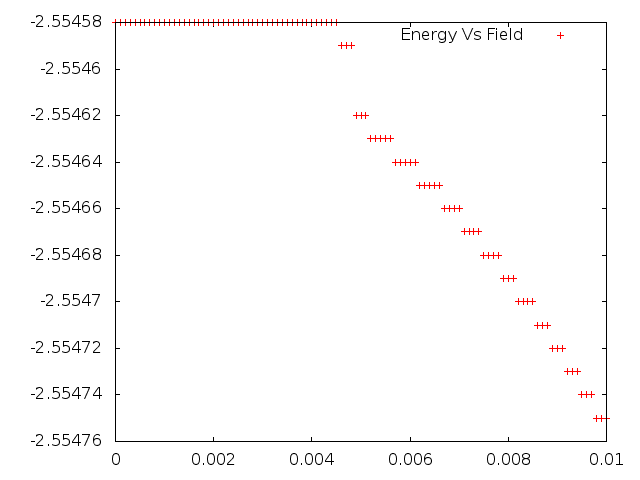
\includegraphics[scale=0.3]{E000to005G.png}
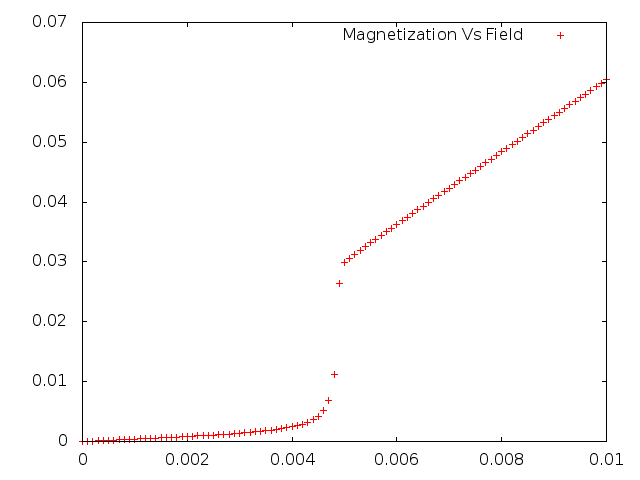
\includegraphics[scale=0.3]{M000to005G.png}
\caption{Energy vs increasing field and Magnetization versus increasing field}
\end{figure}
\begin{figure}[ht]
\centering
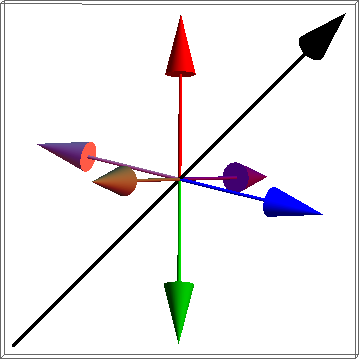
\includegraphics[scale=0.27]{001S000to005G.png}
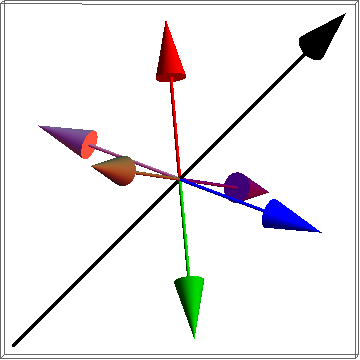
\includegraphics[scale=0.27]{041S000to005G.png}
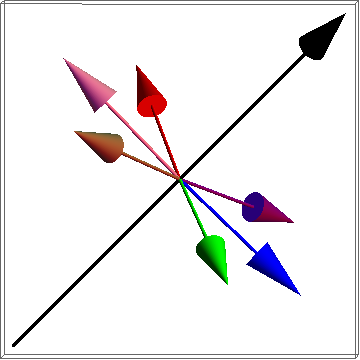
\includegraphics[scale=0.27]{056S000to005G.png}
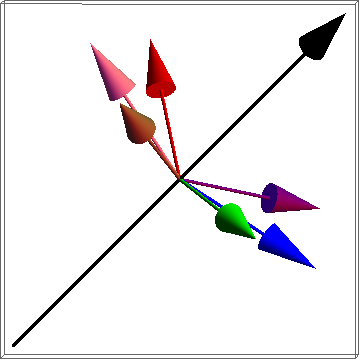
\includegraphics[scale=0.27]{501S000to005G.png}
\caption{Snapshots of the 6 characteristic spins of the lattice at B=0, B=0.0040, B=0.0055, and B=0.05}
\end{figure}
\pagebreak

\begin{figure}
\centering
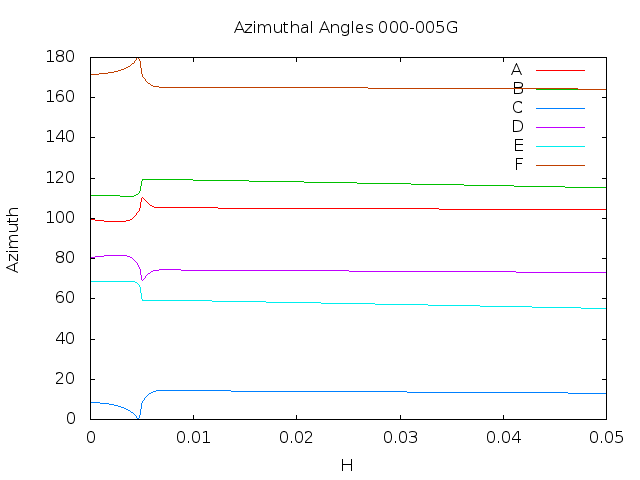
\includegraphics[scale=0.5]{azim000to005G.png}
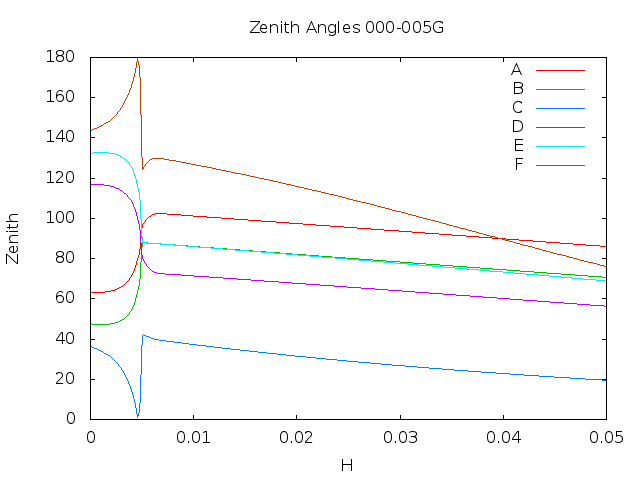
\includegraphics[scale=0.5]{zen000to005G.png}
\caption{The angles are those between a chosen vector lying in the plane intersected by 111,
and a projection of each of the A, B, C, D, E, and F spins. Azimuthal angles are followed by zenith angles.}
\end{figure}
\pagebreak

\begin{center}
\LARGE 0.00 to 0.05 G Spin Chart

 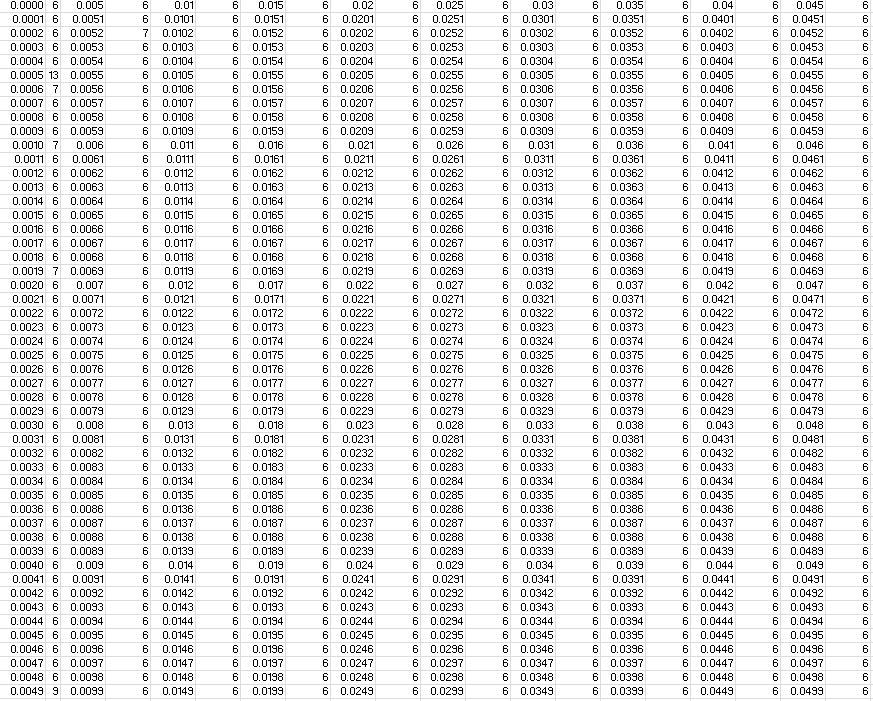
\includegraphics[keepaspectratio,scale=0.7]{000to005SpinChart.png}
\end{center}
\pagebreak
\thispagestyle{plain}
\begin{center}
\LARGE
RUN 2: Decreasing Field, Ground State
\end{center}
\paragraph
\large
No transition is observed in this scenario, similar to the 2000 step case. The spins gradually align with the 111
vector as the field in 111 direction increases. 
\begin{figure}[h]
 \centering 
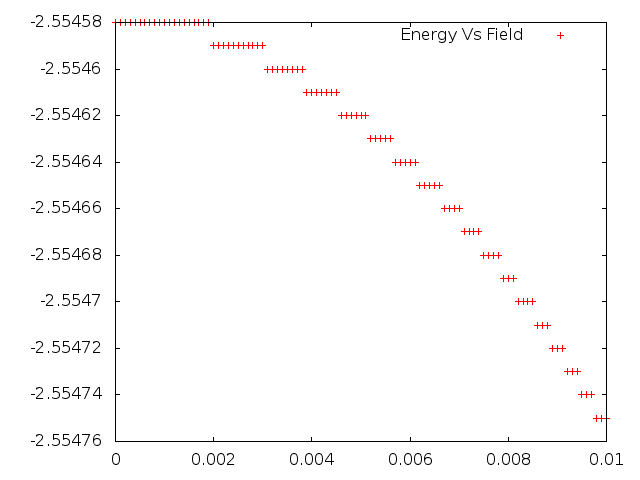
\includegraphics[scale=0.3]{E005to000G.png}
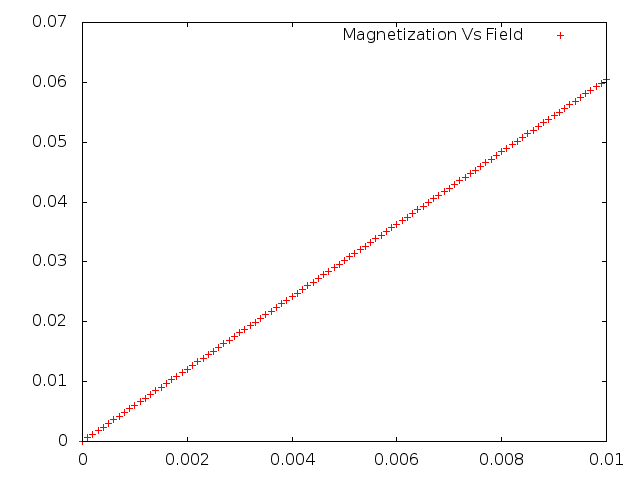
\includegraphics[scale=0.3]{M005to000G.png}
\caption{Energy vs decreasing field and Magnetization versus decreasing field}
\end{figure}
\begin{figure}[ht]
\centering
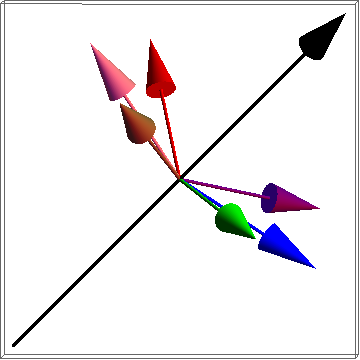
\includegraphics[scale=0.27]{001S005to000G.png}
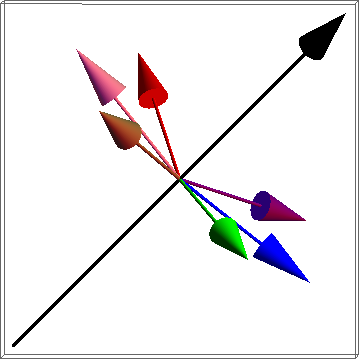
\includegraphics[scale=0.27]{214S005to000G.png}
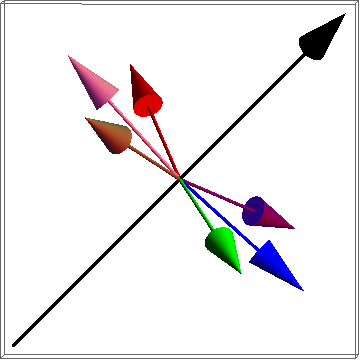
\includegraphics[scale=0.27]{372S005to000G.png}
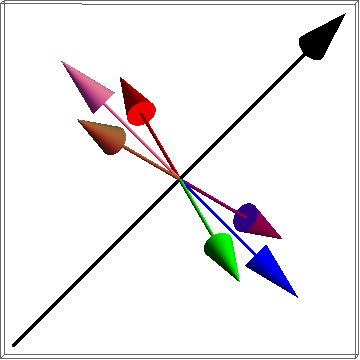
\includegraphics[scale=0.27]{501S005to000G.png}
\caption{Snapshots of the 6 characteristic spins of the lattice at B=0.05, B=0.0287, B=0.0129, and B=0.00}
\end{figure}
\pagebreak
\begin{figure}
\centering
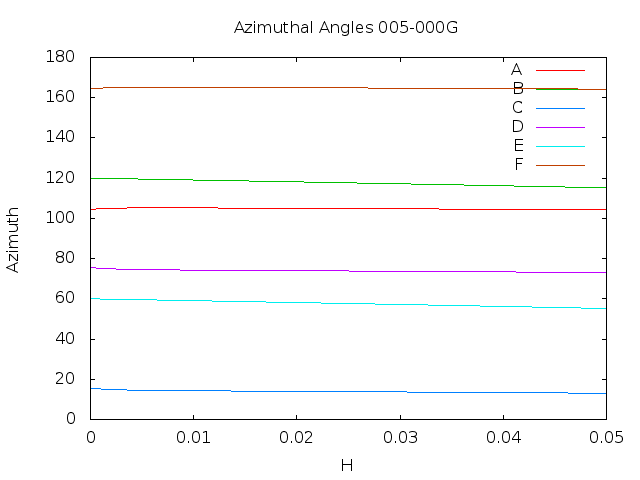
\includegraphics[scale=0.5]{azim005to000G.png}
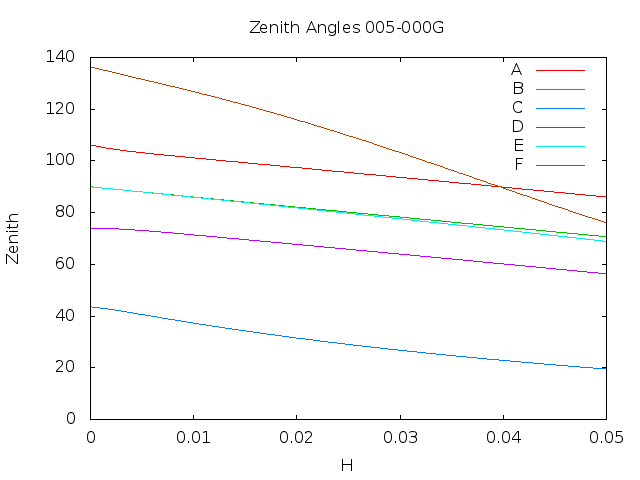
\includegraphics[scale=0.5]{zen005to000G.png}
\caption{The angles are those between a chosen vector lying in the plane intersected by 111,
and a projection of each of the A, B, C, D, E, and F  spins. Azimuthal angles are followed by zenith angles.}
\end{figure}
\pagebreak
\begin{center}
\LARGE 0.05 to 0.00 G Spin Chart
 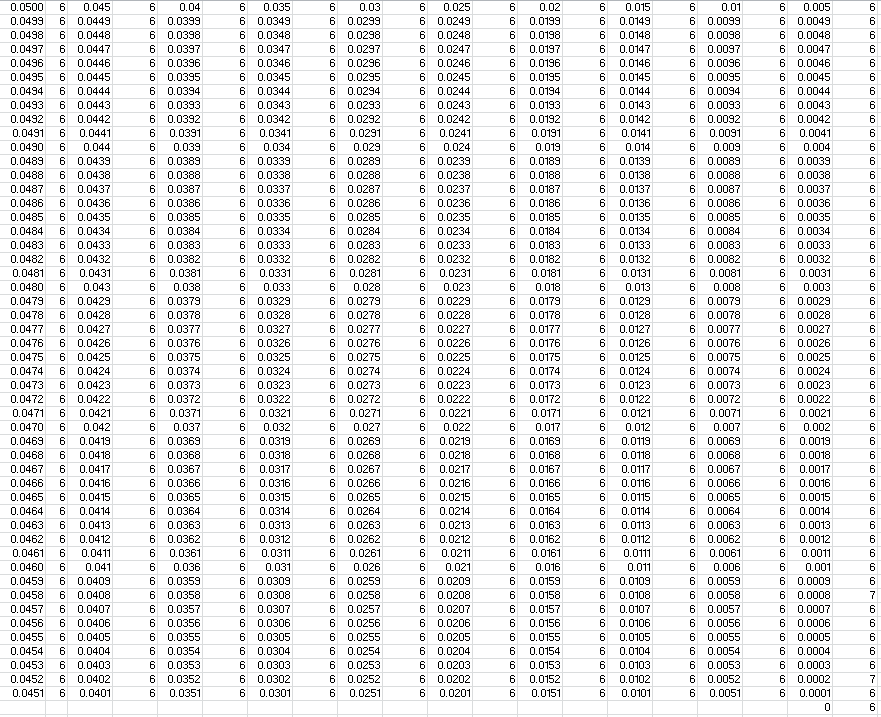
\includegraphics[keepaspectratio,scale=0.7]{005to000SpinChart.png}
\end{center}
\pagebreak

\thispagestyle{plain}
\begin{center}
\LARGE
RUN 3: Increasing Field, Random State
\end{center}
\paragraph
\large
Similar to run 1, a transition to a planar state is observed at around 0.0037.This contrasts the transition field of 
0.49 in the run starting from a ground state. This could be due to the fact the ground state that is initially 
generated at H=0 is slightly different than that of the one used in run 1 and run 2. Maybe there is a relationship
that tells us what field the transition will occur for a given theta and phi?
\begin{figure}[h]
 \centering 
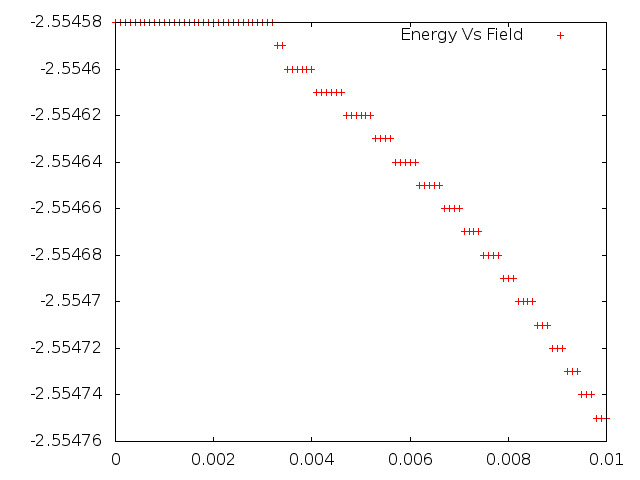
\includegraphics[scale=0.3]{E000to005R.png}
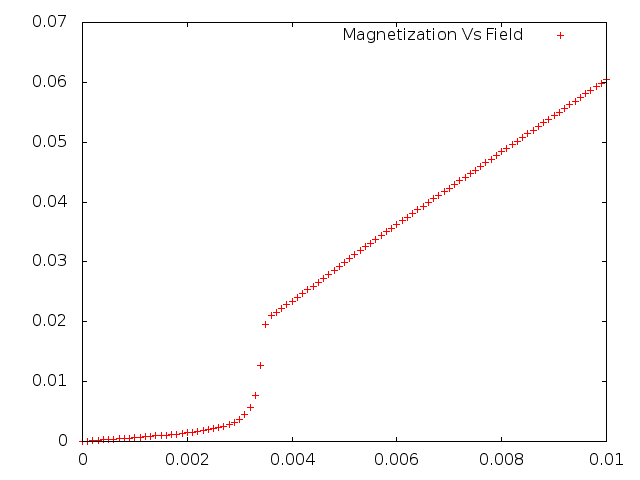
\includegraphics[scale=0.3]{M000to005R.png}
\caption{Energy vs increasing field and Magnetization versus increasing field}
\end{figure}
\begin{figure}[ht]
\centering
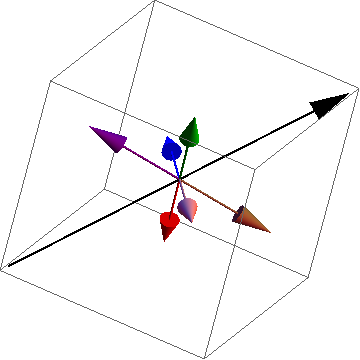
\includegraphics[scale=0.27]{001S000to005R.png}
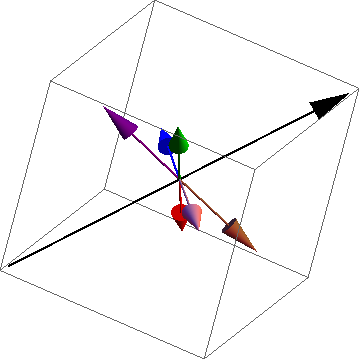
\includegraphics[scale=0.27]{033S000to005R.png}
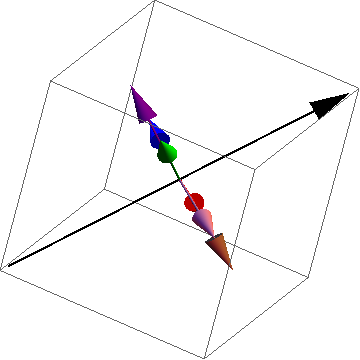
\includegraphics[scale=0.27]{041S000to005R.png}
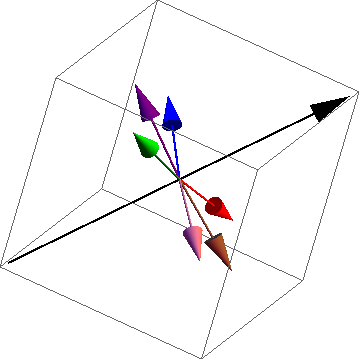
\includegraphics[scale=0.27]{069S000to005R.png}
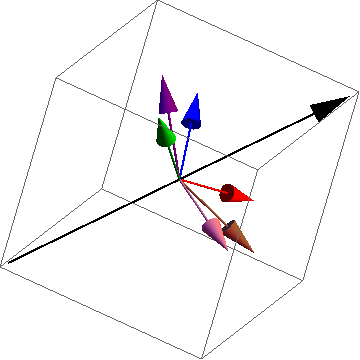
\includegraphics[scale=0.27]{501S000to005R.png}
\caption{Snapshots of the 6 characteristic spins of the lattice at H=0.00, 0.0033, 0.0041, 0.0069, and 0.0500}
\end{figure}
\begin{figure}
\centering
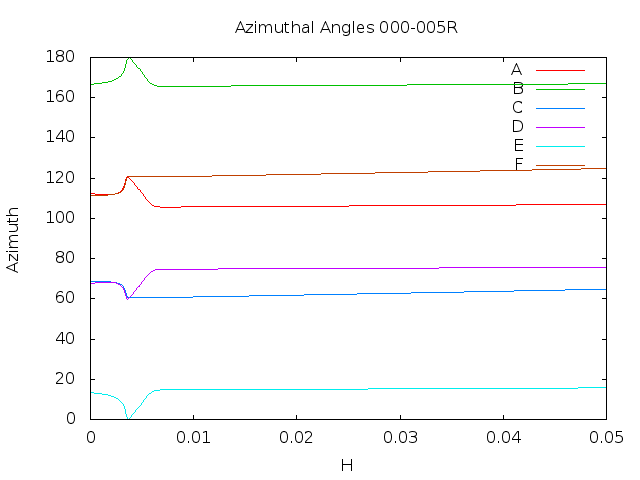
\includegraphics[scale=0.5]{azim000to005R.png}
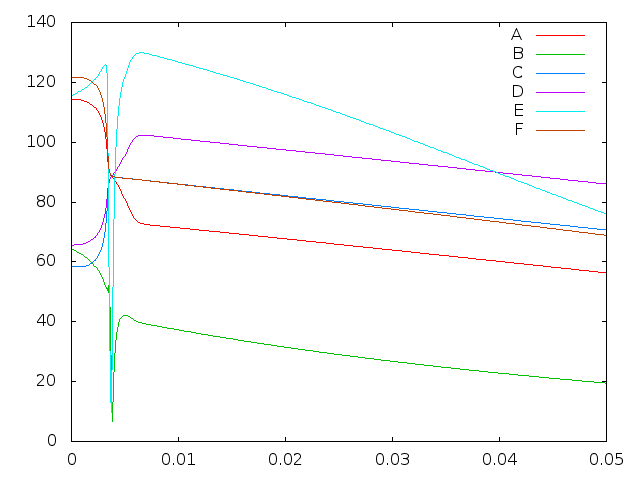
\includegraphics[scale=0.5]{zen000to005R.png}
\caption{The angles are those between a chosen vector lying in the plane intersected by 111,
and a projection of each of the A, B, C, D, E, and F spins. Azimuthal angles are followed by zenith angles.}
\end{figure}
\pagebreak
\begin{center}
\LARGE 0.00 to 0.05 R Spin Chart
 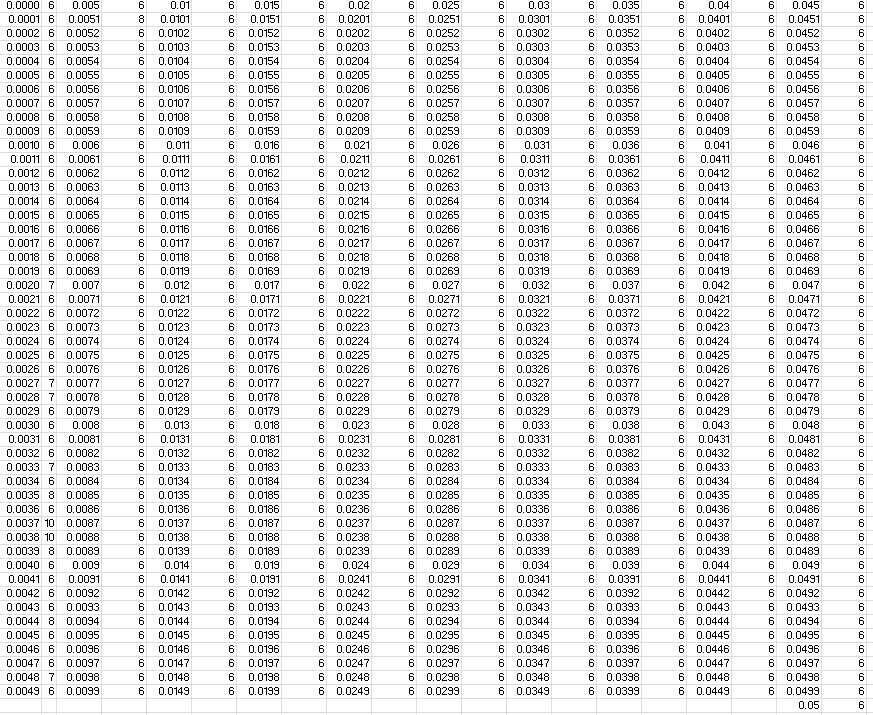
\includegraphics[keepaspectratio,scale=0.7]{000to005RSpinChart.png}
\end{center}
\pagebreak

\thispagestyle{plain}
\begin{center}
\LARGE
RUN 4: Decreasing Field, Random State
\end{center}
\paragraph
\large
Very similar to run 2 in this PDF, but different than run 4 in the April 21st 2016 PDF (2000 steps).
Here, 3000 steps were used and the resulting difference between this and the 2000 step case is the lack of a
transition. It behaves exactly the same way if you were to start from a ground state. 
\begin{figure}[h]
 \centering 
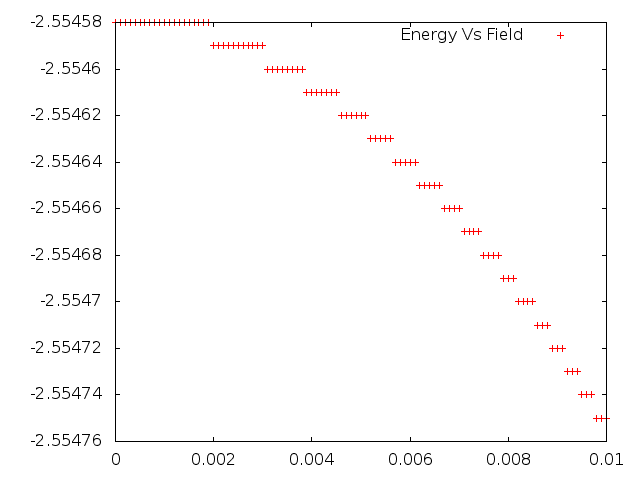
\includegraphics[scale=0.3]{E005to000R.png}
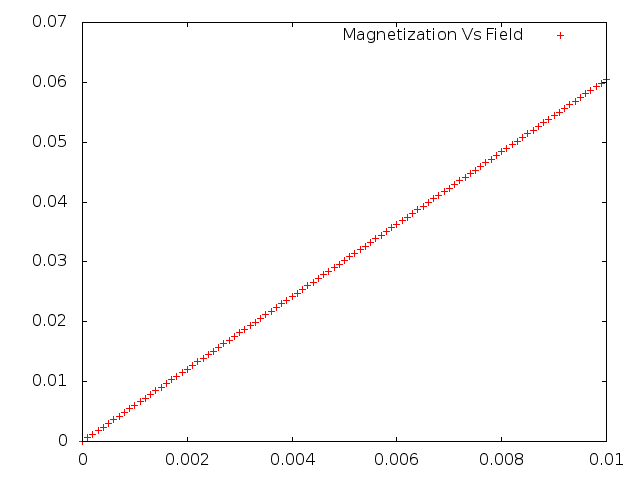
\includegraphics[scale=0.3]{M005to000R.png}
\caption{Energy vs decreasing field and Magnetization versus decreasing field}
\end{figure}
\begin{figure}[ht]
\centering
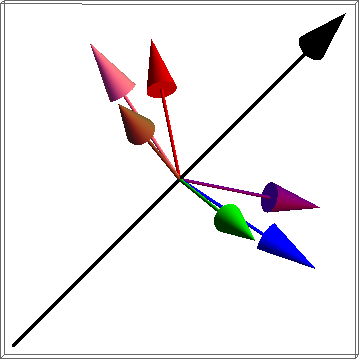
\includegraphics[scale=0.27]{001S005to000R.png}
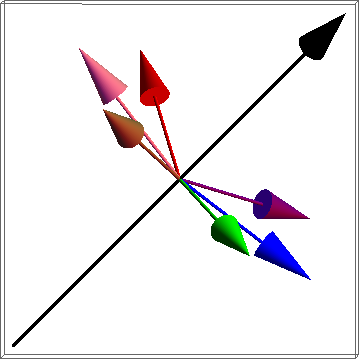
\includegraphics[scale=0.27]{172S005to000R.png}
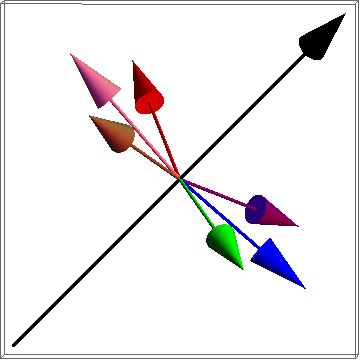
\includegraphics[scale=0.27]{325S005to000R.png}
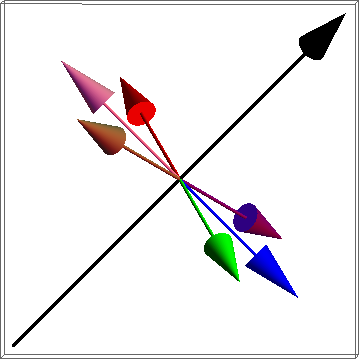
\includegraphics[scale=0.27]{501S005to000R.png}
\caption{Snapshots of the 6 characteristic spins at H=0.05, 0.0329, 0.0176, and 0}
\end{figure}
\pagebreak

\begin{figure}
\centering
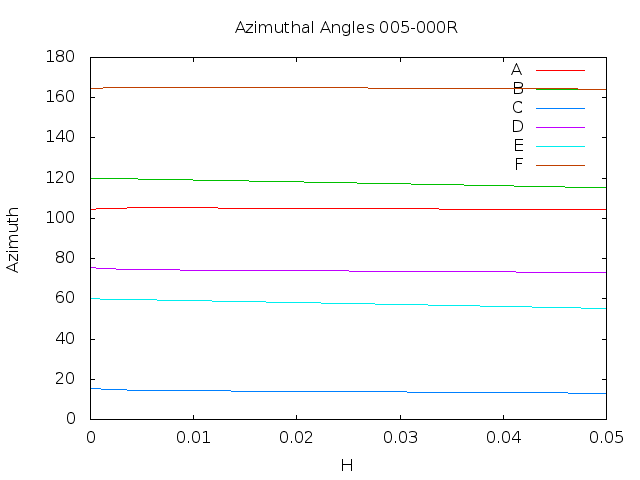
\includegraphics[scale=0.5]{azim005to000R.png}
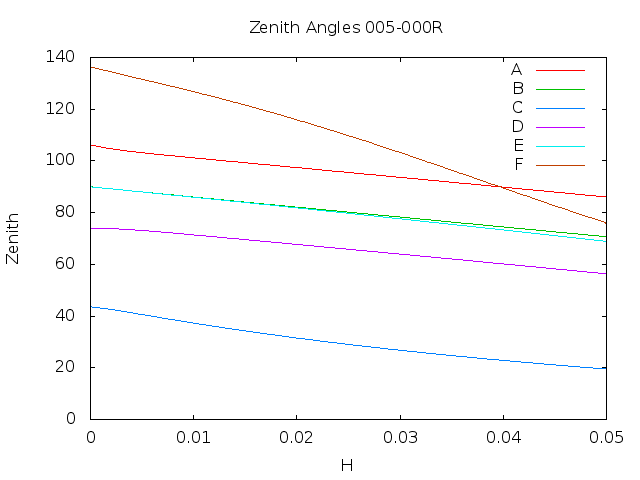
\includegraphics[scale=0.5]{zen005to000R.png}
\caption{The angles are those between a chosen vector lying in the plane intersected by 111,
and a projection of each of the A, B, C, D, E, and F  spins. Azimuthal angles are followed by zenith angles.}
\end{figure}
\pagebreak

\pagebreak
\begin{center}
\LARGE 0.05 to 0.00 R Spin Chart
 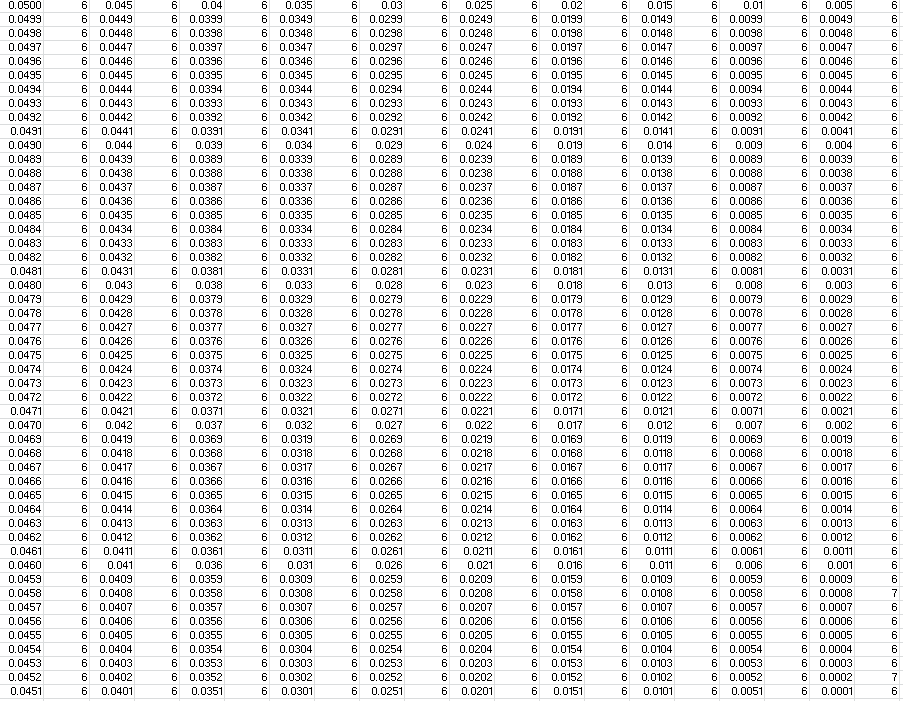
\includegraphics[keepaspectratio,scale=0.7]{005to000RSpinChart.png}
\end{center}
\pagebreak


\begin{center}
\LARGE\textbf{Appendices} \\
\end{center}
\Large
Appendix A - Finding Unique Spins
\large
\paragraph{Overview}
This script is used to find the zenith and azimuth angles of the spins in the 111 plane. I've looked at the calculations
the script makes along the process of finding these angles, and I've manually done them myself. The script performs
the calculations correctly. 
\lstset{language=BASH}
\begin{lstlisting}

#!/bin/bash

#Revision 3 - FOR L=12 ONLY
#May 17th 2016

arccos() {
    scale=17
    if (( $(echo "$1 == 0" | bc -l) )); then
        echo "a(1)*2" | bc -l
    elif (( $(echo "(-1 <= $1) && ($1 < 0)" | bc -l) )); then
        echo "scale=${scale}; a(1)*4 - a(sqrt((1/($1^2))-1))" | bc -l
    elif (( $(echo "(0 < $1) && ($1 <= 1)" | bc -l) )); then
        echo "scale=${scale}; a(sqrt((1/($1^2))-1))" | bc -l
    else
        echo "input out of range"
        return 1
    fi
}


if [[ `cat conf0000.dat | wc -l` -ne 1296 ]];then
echo "Either the conf files are not from L=12 simulations, or conf0000.dat DNE"
echo "Script will fail. Exiting."
exit 1
fi
if [[ -s "debug.txt" ]];then
echo "Resetting debug.txt"
rm debug.txt
fi
PI=3.14159265359
Root3=1.73205080757
Normal="Normals.txt"
perpNorm="NormalPerpendiculars.txt"
if [[ $# < 2 ]];then
echo "usage: script outputFile factor"
exit 1
fi

rm $1
outputFile=$1
rm $outputFile
touch $outputFile
if ! [[ -s $Normal ]];then
echo "Normals.txt DNE. Exiting"
exit 1
fi

if ! [[ -s $perpNorm ]];then
echo "NormalPerpendiculars.txt DNE. Exiting"
exit 1
fi


rm SpinAngles.dat
rm conf[0-9][0-9][0-9][0-9]Angles.dat

#echo "Normal vectors:    1     2     3     4" >> SpinAngles.dat
#echo "Sublattice:  A B C A B C A B C A B C" >> SpinAngles.dat
for f in conf[0-9][0-9][0-9][0-9].dat
do
echo "Processing $f"
#Take name from config file for creation of angle file
name=`echo $f | cut -d '.' -f1`
#EXTRACT SPINS FROM FILE F
length=`cat $f | wc -l`

Spin1=`sed '1q;d' $f`
#echo "Spin1 $Spin1" >> debug.txt

Spin2=`sed '433q;d' $f`
#echo "Spin2 $Spin2" >> debug.txt
Spin3=`sed '865q;d' $f`
#echo "Spin3 $Spin3" >> debug.txt
Spin4=`sed '37q;d' $f`

Spin5=`sed '469q;d' $f`

Spin6=`sed '901q;d' $f`

#DIVIDE FILE ROWS INTO INDIVIDUAL FORMATTED SPINS
spin1x=`echo $Spin1 | awk '{print $1}'`
spin1y=`echo $Spin1 | awk '{print $2}'`
spin1z=`echo $Spin1 | awk '{print $3}'`
spin2x=`echo $Spin2 | awk '{print $1}'`
spin2y=`echo $Spin2 | awk '{print $2}'`
spin2z=`echo $Spin2 | awk '{print $3}'`
spin3x=`echo $Spin3 | awk '{print $1}'`
spin3y=`echo $Spin3 | awk '{print $2}'`
spin3z=`echo $Spin3 | awk '{print $3}'`
spin4x=`echo $Spin4 | awk '{print $1}'`
spin4y=`echo $Spin4 | awk '{print $2}'`
spin4z=`echo $Spin4 | awk '{print $3}'`
spin5x=`echo $Spin5 | awk '{print $1}'`
spin5y=`echo $Spin5 | awk '{print $2}'`
spin5z=`echo $Spin5 | awk '{print $3}'`
spin6x=`echo $Spin6 | awk '{print $1}'`
spin6y=`echo $Spin6 | awk '{print $2}'`
spin6z=`echo $Spin6 | awk '{print $3}'`

spin1x=`printf '%.17f' $spin1x`
spin1y=`printf '%.17f' $spin1y`
spin1z=`printf '%.17f' $spin1z`
spin2x=`printf '%.17f' $spin2x`
spin2y=`printf '%.17f' $spin2y`
spin2z=`printf '%.17f' $spin2z`
spin3x=`printf '%.17f' $spin3x`
spin3y=`printf '%.17f' $spin3y`
spin3z=`printf '%.17f' $spin3z`
spin4x=`printf '%.17f' $spin4x`
spin4y=`printf '%.17f' $spin4y`
spin4z=`printf '%.17f' $spin4z`
spin5x=`printf '%.17f' $spin5x`
spin5y=`printf '%.17f' $spin5y`
spin5z=`printf '%.17f' $spin5z`
spin6x=`printf '%.17f' $spin6x`
spin6y=`printf '%.17f' $spin6y`
spin6z=`printf '%.17f' $spin6z`



#echo $spin1x $spin1y $spin1z $spin2x $spin2y $spin2z $spin3x $spin3y $spin3z
AppendedString=""
#CALCULATION OF ANGLES
NumNorms=`cat Normals.txt | wc -l`

for i in `seq 0 $(($NumNorms/3-1))`; 
do

#Two vectors which are read from two separate files. These vectors need to be orthogonal. 
a=$((1+3*$i))
b=$((2+3*$i))
c=$((3+3*$i))
pa=$((1+3*$i))
pb=$((2+3*$i))
pc=$((3+3*$i))
#Break each vector up into components. 

normx=`cat $Normal | head -n $a | tail -n 1`
normy=`cat $Normal | head -n $b | tail -n 1`
normz=`cat $Normal | head -n $c | tail -n 1`
pnormx=`cat $perpNorm | head -n $pa | tail -n 1`
pnormy=`cat $perpNorm | head -n $pb | tail -n 1`
pnormz=`cat $perpNorm | head -n $pc | tail -n 1`
#echo "$normx $normy $normz $pnormx $pnormy $pnormz" >> debug.txt


#echo "Normal: $normx $normy $normz" >> debug.txt
#echo "Perpendicular normal: $pnormx $pnormy $pnormz" >> debug.txt
#Find the dot product between each spin and the normal vector 
Dot1=`echo "$spin1x*$normx+$spin1y*$normy+$spin1z*$normz" | bc -l`
Dot2=`echo "$spin2x*$normx+$spin2y*$normy+$spin2z*$normz" | bc -l`
Dot3=`echo "$spin3x*$normx+$spin3y*$normy+$spin3z*$normz" | bc -l`
Dot4=`echo "$spin4x*$normx+$spin4y*$normy+$spin4z*$normz" | bc -l`
Dot5=`echo "$spin5x*$normx+$spin5y*$normy+$spin5z*$normz" | bc -l`
Dot6=`echo "$spin6x*$normx+$spin6y*$normy+$spin6z*$normz" | bc -l`
#echo "Dots $Dot1 $Dot2 $Dot3 $Dot4 $Dot5 $Dot6" >> debug.txt
#Find the length of each spin (should just be 1)
Length1=`echo "sqrt($spin1x*$spin1x+$spin1y*$spin1y+$spin1z*$spin1z)" | bc -l`
Length2=`echo "sqrt($spin2x*$spin2x+$spin2y*$spin2y+$spin2z*$spin2z)" | bc -l`
Length3=`echo "sqrt($spin3x*$spin3x+$spin3y*$spin3y+$spin3z*$spin3z)" | bc -l`
Length4=`echo "sqrt($spin4x*$spin4x+$spin4y*$spin4y+$spin4z*$spin4z)" | bc -l`
Length5=`echo "sqrt($spin5x*$spin5x+$spin5y*$spin5y+$spin5z*$spin5z)" | bc -l`
Length6=`echo "sqrt($spin6x*$spin6x+$spin6y*$spin6y+$spin6z*$spin6z)" | bc -l`
#Find the length of each normal vector.
normLen=`echo "sqrt($normx*$normx+$normy*$normy+$normz*$normz)" | bc -l`
pnormLen=`echo "sqrt($pnormx*$pnormx+$pnormy*$pnormy+$pnormz*$pnormz)" | bc -l`
#echo "normlen $normLen pnormLen $pnormLen" >> debug.txt
#echo "Lengths $Length1 $Length2 $Length3" >> debug.txt
#Find the projection of each spin into the plane with normal vector norm
proj1x=`echo "$spin1x - $normx*$Dot1/($normLen*$normLen)" | bc -l`
proj1y=`echo "$spin1y - $normy*$Dot1/($normLen*$normLen)" | bc -l`
proj1z=`echo "$spin1z - $normz*$Dot1/($normLen*$normLen)" | bc -l`
#echo "proj1 $proj1x $proj1y $proj1z" >> debug.txt
proj2x=`echo "$spin2x - $normx*$Dot2/($normLen*$normLen)" | bc -l`
proj2y=`echo "$spin2y - $normy*$Dot2/($normLen*$normLen)" | bc -l`
proj2z=`echo "$spin2z - $normz*$Dot2/($normLen*$normLen)" | bc -l`
#echo "proj2 $proj2x $proj2y $proj2z" >> debug.txt
proj3x=`echo "$spin3x - $normx*$Dot3/($normLen*$normLen)" | bc -l`
proj3y=`echo "$spin3y - $normy*$Dot3/($normLen*$normLen)" | bc -l`
proj3z=`echo "$spin3z - $normz*$Dot3/($normLen*$normLen)" | bc -l`
#echo "proj3 $proj3x $proj3y $proj3z" >> debug.txt
proj4x=`echo "$spin4x - $normx*$Dot4/($normLen*$normLen)" | bc -l`
proj4y=`echo "$spin4y - $normy*$Dot4/($normLen*$normLen)" | bc -l`
proj4z=`echo "$spin4z - $normz*$Dot4/($normLen*$normLen)" | bc -l`
#echo "proj4 $proj4x $proj4y $proj4z" >> debug.txt
proj5x=`echo "$spin5x - $normx*$Dot5/($normLen*$normLen)" | bc -l`
proj5y=`echo "$spin5y - $normy*$Dot5/($normLen*$normLen)" | bc -l`
proj5z=`echo "$spin5z - $normz*$Dot5/($normLen*$normLen)" | bc -l`
#echo "proj5 $proj5x $proj5y $proj5z" >> debug.txt
proj6x=`echo "$spin6x - $normx*$Dot6/($normLen*$normLen)" | bc -l`
proj6y=`echo "$spin6y - $normy*$Dot6/($normLen*$normLen)" | bc -l`
proj6z=`echo "$spin6z - $normz*$Dot6/($normLen*$normLen)" | bc -l`
#echo "proj6 $proj6x $proj6y $proj6z" >> debug.txt

#Find the dot product between each projected spin and pnorm
proj1Dot=`echo "$proj1x*$pnormx+$proj1y*$pnormy+$proj1z*$pnormz" | bc -l`
proj2Dot=`echo "$proj2x*$pnormx+$proj2y*$pnormy+$proj2z*$pnormz" | bc -l`
proj3Dot=`echo "$proj3x*$pnormx+$proj3y*$pnormy+$proj3z*$pnormz" | bc -l`
proj4Dot=`echo "$proj4x*$pnormx+$proj4y*$pnormy+$proj4z*$pnormz" | bc -l`
proj5Dot=`echo "$proj5x*$pnormx+$proj5y*$pnormy+$proj5z*$pnormz" | bc -l`
proj6Dot=`echo "$proj6x*$pnormx+$proj6y*$pnormy+$proj6z*$pnormz" | bc -l`
#echo "projDots $proj1Dot $proj2Dot $proj3Dot $proj4Dot $proj5Dot $proj6Dot" >> debug.txt
#Find the length of each projected spin
proj1Len=`echo "sqrt($proj1x*$proj1x+$proj1y*$proj1y+$proj1z*$proj1z)" | bc -l`
proj2Len=`echo "sqrt($proj2x*$proj2x+$proj2y*$proj2y+$proj2z*$proj2z)" | bc -l`
proj3Len=`echo "sqrt($proj3x*$proj3x+$proj3y*$proj3y+$proj3z*$proj3z)" | bc -l`
proj4Len=`echo "sqrt($proj4x*$proj4x+$proj4y*$proj4y+$proj4z*$proj4z)" | bc -l`
proj5Len=`echo "sqrt($proj5x*$proj5x+$proj5y*$proj5y+$proj5z*$proj5z)" | bc -l`
proj6Len=`echo "sqrt($proj6x*$proj6x+$proj6y*$proj6y+$proj6z*$proj6z)" | bc -l`
#echo "ProjLengths $proj1Len $proj2Len $proj3Len" >> debug.txt
#Calculate projDOTpnorm/[Length(proj)*Length(pnorm)]
#This will be used to find the angle by taking the arccos of this value
tmp1=`echo "$proj1Dot/($proj1Len*$pnormLen)" | bc -l`
tmp2=`echo "$proj2Dot/($proj2Len*$pnormLen)" | bc -l`
tmp3=`echo "$proj3Dot/($proj3Len*$pnormLen)" | bc -l`
tmp4=`echo "$proj4Dot/($proj4Len*$pnormLen)" | bc -l`
tmp5=`echo "$proj5Dot/($proj5Len*$pnormLen)" | bc -l`
tmp6=`echo "$proj6Dot/($proj6Len*$pnormLen)" | bc -l`
#echo 'Dots/Length' ${Angle1:0:9} ${Angle2:0:9} ${Angle3:0:9}
#echo "Cos(Angles) $tmp1 $tmp2 $tmp3 $tmp4 $tmp5 $tmp6" >> debug.txt
radAng1=`arccos $tmp1`
radAng2=`arccos $tmp2`
radAng3=`arccos $tmp3`
radAng4=`arccos $tmp4`
radAng5=`arccos $tmp5`
radAng6=`arccos $tmp6`
#echo "radAngs $radAng1 $radAng2 $radAng3 $radAng4 $radAng5 $radAng6" >> debug.txt
Angle1=`echo "$radAng1*180/$PI" | bc -l`
Angle2=`echo "$radAng2*180/$PI" | bc -l`
Angle3=`echo "$radAng3*180/$PI" | bc -l`
Angle4=`echo "$radAng4*180/$PI" | bc -l`
Angle5=`echo "$radAng5*180/$PI" | bc -l`
Angle6=`echo "$radAng6*180/$PI" | bc -l`
#echo "Final Angles $Angle1 $Angle2 $Angle3 $Angle4 $Angle5 $Angle6" >> debug.txt
#echo 'Final Angles' ${Angle1:0:9} ${Angle2:0:9} ${Angle3:0:9}
#Angle1=`echo $Angle1 | tr -d '-'`
#Angle2=`echo $Angle2 | tr -d '-'`
#Angle3=`echo $Angle3 | tr -d '-'`
#echo "Angles without negatives" ${Angle1:0:9} ${Angle2:0:9} ${Angle3:0:9}
AppendedString="$AppendedString ${Angle1:0:9} ${Angle2:0:9} ${Angle3:0:9} ${Angle4:0:9} ${Angle5:0:9} ${Angle6:0:9}"
done

fnum=`echo $f | grep -o "[0-9][0-9][0-9][0-9]"`
fnum=`echo "0.05 - $fnum/$2" | bc -l` 
echo $fnum $AppendedString >> $outputFile
done

#Revision History
#Revision 1 November 24th 2015
#Read in normal vector components from text file. Use them to find the dot product
#between the normal vector and the 3 spins each located at lines 1, 433, and 865.
#The files containing the spins are almost always structured such that spin A repeats
#followed by the negative of A. This repition continues with +A followed by -A for a number
#of times. The same happens for +B and -B, and +C and -C. The lines at which B begins to appear
#is line 433, and the line at which C begins to appear is 865. This is why it is chosen. 
#Rev 2?
#Rev 3 Finds the angles of all 6 spins

\end{lstlisting}
\end{document}